
% Default to the notebook output style

    


% Inherit from the specified cell style.




    
\documentclass[11pt]{article}

    
    
    \usepackage[T1]{fontenc}
    % Nicer default font (+ math font) than Computer Modern for most use cases
    \usepackage{mathpazo}

    % Basic figure setup, for now with no caption control since it's done
    % automatically by Pandoc (which extracts ![](path) syntax from Markdown).
    \usepackage{graphicx}
    % We will generate all images so they have a width \maxwidth. This means
    % that they will get their normal width if they fit onto the page, but
    % are scaled down if they would overflow the margins.
    \makeatletter
    \def\maxwidth{\ifdim\Gin@nat@width>\linewidth\linewidth
    \else\Gin@nat@width\fi}
    \makeatother
    \let\Oldincludegraphics\includegraphics
    % Set max figure width to be 80% of text width, for now hardcoded.
    \renewcommand{\includegraphics}[1]{\Oldincludegraphics[width=.8\maxwidth]{#1}}
    % Ensure that by default, figures have no caption (until we provide a
    % proper Figure object with a Caption API and a way to capture that
    % in the conversion process - todo).
    \usepackage{caption}
    \DeclareCaptionLabelFormat{nolabel}{}
    \captionsetup{labelformat=nolabel}

    \usepackage{adjustbox} % Used to constrain images to a maximum size 
    \usepackage{xcolor} % Allow colors to be defined
    \usepackage{enumerate} % Needed for markdown enumerations to work
    \usepackage{geometry} % Used to adjust the document margins
    \usepackage{amsmath} % Equations
    \usepackage{amssymb} % Equations
    \usepackage{textcomp} % defines textquotesingle
    % Hack from http://tex.stackexchange.com/a/47451/13684:
    \AtBeginDocument{%
        \def\PYZsq{\textquotesingle}% Upright quotes in Pygmentized code
    }
    \usepackage{upquote} % Upright quotes for verbatim code
    \usepackage{eurosym} % defines \euro
    \usepackage[mathletters]{ucs} % Extended unicode (utf-8) support
    \usepackage[utf8x]{inputenc} % Allow utf-8 characters in the tex document
    \usepackage{fancyvrb} % verbatim replacement that allows latex
    \usepackage{grffile} % extends the file name processing of package graphics 
                         % to support a larger range 
    % The hyperref package gives us a pdf with properly built
    % internal navigation ('pdf bookmarks' for the table of contents,
    % internal cross-reference links, web links for URLs, etc.)
    \usepackage{hyperref}
    \usepackage{longtable} % longtable support required by pandoc >1.10
    \usepackage{booktabs}  % table support for pandoc > 1.12.2
    \usepackage[inline]{enumitem} % IRkernel/repr support (it uses the enumerate* environment)
    \usepackage[normalem]{ulem} % ulem is needed to support strikethroughs (\sout)
                                % normalem makes italics be italics, not underlines
    

    
    
    % Colors for the hyperref package
    \definecolor{urlcolor}{rgb}{0,.145,.698}
    \definecolor{linkcolor}{rgb}{.71,0.21,0.01}
    \definecolor{citecolor}{rgb}{.12,.54,.11}

    % ANSI colors
    \definecolor{ansi-black}{HTML}{3E424D}
    \definecolor{ansi-black-intense}{HTML}{282C36}
    \definecolor{ansi-red}{HTML}{E75C58}
    \definecolor{ansi-red-intense}{HTML}{B22B31}
    \definecolor{ansi-green}{HTML}{00A250}
    \definecolor{ansi-green-intense}{HTML}{007427}
    \definecolor{ansi-yellow}{HTML}{DDB62B}
    \definecolor{ansi-yellow-intense}{HTML}{B27D12}
    \definecolor{ansi-blue}{HTML}{208FFB}
    \definecolor{ansi-blue-intense}{HTML}{0065CA}
    \definecolor{ansi-magenta}{HTML}{D160C4}
    \definecolor{ansi-magenta-intense}{HTML}{A03196}
    \definecolor{ansi-cyan}{HTML}{60C6C8}
    \definecolor{ansi-cyan-intense}{HTML}{258F8F}
    \definecolor{ansi-white}{HTML}{C5C1B4}
    \definecolor{ansi-white-intense}{HTML}{A1A6B2}

    % commands and environments needed by pandoc snippets
    % extracted from the output of `pandoc -s`
    \providecommand{\tightlist}{%
      \setlength{\itemsep}{0pt}\setlength{\parskip}{0pt}}
    \DefineVerbatimEnvironment{Highlighting}{Verbatim}{commandchars=\\\{\}}
    % Add ',fontsize=\small' for more characters per line
    \newenvironment{Shaded}{}{}
    \newcommand{\KeywordTok}[1]{\textcolor[rgb]{0.00,0.44,0.13}{\textbf{{#1}}}}
    \newcommand{\DataTypeTok}[1]{\textcolor[rgb]{0.56,0.13,0.00}{{#1}}}
    \newcommand{\DecValTok}[1]{\textcolor[rgb]{0.25,0.63,0.44}{{#1}}}
    \newcommand{\BaseNTok}[1]{\textcolor[rgb]{0.25,0.63,0.44}{{#1}}}
    \newcommand{\FloatTok}[1]{\textcolor[rgb]{0.25,0.63,0.44}{{#1}}}
    \newcommand{\CharTok}[1]{\textcolor[rgb]{0.25,0.44,0.63}{{#1}}}
    \newcommand{\StringTok}[1]{\textcolor[rgb]{0.25,0.44,0.63}{{#1}}}
    \newcommand{\CommentTok}[1]{\textcolor[rgb]{0.38,0.63,0.69}{\textit{{#1}}}}
    \newcommand{\OtherTok}[1]{\textcolor[rgb]{0.00,0.44,0.13}{{#1}}}
    \newcommand{\AlertTok}[1]{\textcolor[rgb]{1.00,0.00,0.00}{\textbf{{#1}}}}
    \newcommand{\FunctionTok}[1]{\textcolor[rgb]{0.02,0.16,0.49}{{#1}}}
    \newcommand{\RegionMarkerTok}[1]{{#1}}
    \newcommand{\ErrorTok}[1]{\textcolor[rgb]{1.00,0.00,0.00}{\textbf{{#1}}}}
    \newcommand{\NormalTok}[1]{{#1}}
    
    % Additional commands for more recent versions of Pandoc
    \newcommand{\ConstantTok}[1]{\textcolor[rgb]{0.53,0.00,0.00}{{#1}}}
    \newcommand{\SpecialCharTok}[1]{\textcolor[rgb]{0.25,0.44,0.63}{{#1}}}
    \newcommand{\VerbatimStringTok}[1]{\textcolor[rgb]{0.25,0.44,0.63}{{#1}}}
    \newcommand{\SpecialStringTok}[1]{\textcolor[rgb]{0.73,0.40,0.53}{{#1}}}
    \newcommand{\ImportTok}[1]{{#1}}
    \newcommand{\DocumentationTok}[1]{\textcolor[rgb]{0.73,0.13,0.13}{\textit{{#1}}}}
    \newcommand{\AnnotationTok}[1]{\textcolor[rgb]{0.38,0.63,0.69}{\textbf{\textit{{#1}}}}}
    \newcommand{\CommentVarTok}[1]{\textcolor[rgb]{0.38,0.63,0.69}{\textbf{\textit{{#1}}}}}
    \newcommand{\VariableTok}[1]{\textcolor[rgb]{0.10,0.09,0.49}{{#1}}}
    \newcommand{\ControlFlowTok}[1]{\textcolor[rgb]{0.00,0.44,0.13}{\textbf{{#1}}}}
    \newcommand{\OperatorTok}[1]{\textcolor[rgb]{0.40,0.40,0.40}{{#1}}}
    \newcommand{\BuiltInTok}[1]{{#1}}
    \newcommand{\ExtensionTok}[1]{{#1}}
    \newcommand{\PreprocessorTok}[1]{\textcolor[rgb]{0.74,0.48,0.00}{{#1}}}
    \newcommand{\AttributeTok}[1]{\textcolor[rgb]{0.49,0.56,0.16}{{#1}}}
    \newcommand{\InformationTok}[1]{\textcolor[rgb]{0.38,0.63,0.69}{\textbf{\textit{{#1}}}}}
    \newcommand{\WarningTok}[1]{\textcolor[rgb]{0.38,0.63,0.69}{\textbf{\textit{{#1}}}}}
    
    
    % Define a nice break command that doesn't care if a line doesn't already
    % exist.
    \def\br{\hspace*{\fill} \\* }
    % Math Jax compatability definitions
    \def\gt{>}
    \def\lt{<}
    % Document parameters
    \title{task01-initial-topic-investigation}
    
    
    

    % Pygments definitions
    
\makeatletter
\def\PY@reset{\let\PY@it=\relax \let\PY@bf=\relax%
    \let\PY@ul=\relax \let\PY@tc=\relax%
    \let\PY@bc=\relax \let\PY@ff=\relax}
\def\PY@tok#1{\csname PY@tok@#1\endcsname}
\def\PY@toks#1+{\ifx\relax#1\empty\else%
    \PY@tok{#1}\expandafter\PY@toks\fi}
\def\PY@do#1{\PY@bc{\PY@tc{\PY@ul{%
    \PY@it{\PY@bf{\PY@ff{#1}}}}}}}
\def\PY#1#2{\PY@reset\PY@toks#1+\relax+\PY@do{#2}}

\expandafter\def\csname PY@tok@w\endcsname{\def\PY@tc##1{\textcolor[rgb]{0.73,0.73,0.73}{##1}}}
\expandafter\def\csname PY@tok@c\endcsname{\let\PY@it=\textit\def\PY@tc##1{\textcolor[rgb]{0.25,0.50,0.50}{##1}}}
\expandafter\def\csname PY@tok@cp\endcsname{\def\PY@tc##1{\textcolor[rgb]{0.74,0.48,0.00}{##1}}}
\expandafter\def\csname PY@tok@k\endcsname{\let\PY@bf=\textbf\def\PY@tc##1{\textcolor[rgb]{0.00,0.50,0.00}{##1}}}
\expandafter\def\csname PY@tok@kp\endcsname{\def\PY@tc##1{\textcolor[rgb]{0.00,0.50,0.00}{##1}}}
\expandafter\def\csname PY@tok@kt\endcsname{\def\PY@tc##1{\textcolor[rgb]{0.69,0.00,0.25}{##1}}}
\expandafter\def\csname PY@tok@o\endcsname{\def\PY@tc##1{\textcolor[rgb]{0.40,0.40,0.40}{##1}}}
\expandafter\def\csname PY@tok@ow\endcsname{\let\PY@bf=\textbf\def\PY@tc##1{\textcolor[rgb]{0.67,0.13,1.00}{##1}}}
\expandafter\def\csname PY@tok@nb\endcsname{\def\PY@tc##1{\textcolor[rgb]{0.00,0.50,0.00}{##1}}}
\expandafter\def\csname PY@tok@nf\endcsname{\def\PY@tc##1{\textcolor[rgb]{0.00,0.00,1.00}{##1}}}
\expandafter\def\csname PY@tok@nc\endcsname{\let\PY@bf=\textbf\def\PY@tc##1{\textcolor[rgb]{0.00,0.00,1.00}{##1}}}
\expandafter\def\csname PY@tok@nn\endcsname{\let\PY@bf=\textbf\def\PY@tc##1{\textcolor[rgb]{0.00,0.00,1.00}{##1}}}
\expandafter\def\csname PY@tok@ne\endcsname{\let\PY@bf=\textbf\def\PY@tc##1{\textcolor[rgb]{0.82,0.25,0.23}{##1}}}
\expandafter\def\csname PY@tok@nv\endcsname{\def\PY@tc##1{\textcolor[rgb]{0.10,0.09,0.49}{##1}}}
\expandafter\def\csname PY@tok@no\endcsname{\def\PY@tc##1{\textcolor[rgb]{0.53,0.00,0.00}{##1}}}
\expandafter\def\csname PY@tok@nl\endcsname{\def\PY@tc##1{\textcolor[rgb]{0.63,0.63,0.00}{##1}}}
\expandafter\def\csname PY@tok@ni\endcsname{\let\PY@bf=\textbf\def\PY@tc##1{\textcolor[rgb]{0.60,0.60,0.60}{##1}}}
\expandafter\def\csname PY@tok@na\endcsname{\def\PY@tc##1{\textcolor[rgb]{0.49,0.56,0.16}{##1}}}
\expandafter\def\csname PY@tok@nt\endcsname{\let\PY@bf=\textbf\def\PY@tc##1{\textcolor[rgb]{0.00,0.50,0.00}{##1}}}
\expandafter\def\csname PY@tok@nd\endcsname{\def\PY@tc##1{\textcolor[rgb]{0.67,0.13,1.00}{##1}}}
\expandafter\def\csname PY@tok@s\endcsname{\def\PY@tc##1{\textcolor[rgb]{0.73,0.13,0.13}{##1}}}
\expandafter\def\csname PY@tok@sd\endcsname{\let\PY@it=\textit\def\PY@tc##1{\textcolor[rgb]{0.73,0.13,0.13}{##1}}}
\expandafter\def\csname PY@tok@si\endcsname{\let\PY@bf=\textbf\def\PY@tc##1{\textcolor[rgb]{0.73,0.40,0.53}{##1}}}
\expandafter\def\csname PY@tok@se\endcsname{\let\PY@bf=\textbf\def\PY@tc##1{\textcolor[rgb]{0.73,0.40,0.13}{##1}}}
\expandafter\def\csname PY@tok@sr\endcsname{\def\PY@tc##1{\textcolor[rgb]{0.73,0.40,0.53}{##1}}}
\expandafter\def\csname PY@tok@ss\endcsname{\def\PY@tc##1{\textcolor[rgb]{0.10,0.09,0.49}{##1}}}
\expandafter\def\csname PY@tok@sx\endcsname{\def\PY@tc##1{\textcolor[rgb]{0.00,0.50,0.00}{##1}}}
\expandafter\def\csname PY@tok@m\endcsname{\def\PY@tc##1{\textcolor[rgb]{0.40,0.40,0.40}{##1}}}
\expandafter\def\csname PY@tok@gh\endcsname{\let\PY@bf=\textbf\def\PY@tc##1{\textcolor[rgb]{0.00,0.00,0.50}{##1}}}
\expandafter\def\csname PY@tok@gu\endcsname{\let\PY@bf=\textbf\def\PY@tc##1{\textcolor[rgb]{0.50,0.00,0.50}{##1}}}
\expandafter\def\csname PY@tok@gd\endcsname{\def\PY@tc##1{\textcolor[rgb]{0.63,0.00,0.00}{##1}}}
\expandafter\def\csname PY@tok@gi\endcsname{\def\PY@tc##1{\textcolor[rgb]{0.00,0.63,0.00}{##1}}}
\expandafter\def\csname PY@tok@gr\endcsname{\def\PY@tc##1{\textcolor[rgb]{1.00,0.00,0.00}{##1}}}
\expandafter\def\csname PY@tok@ge\endcsname{\let\PY@it=\textit}
\expandafter\def\csname PY@tok@gs\endcsname{\let\PY@bf=\textbf}
\expandafter\def\csname PY@tok@gp\endcsname{\let\PY@bf=\textbf\def\PY@tc##1{\textcolor[rgb]{0.00,0.00,0.50}{##1}}}
\expandafter\def\csname PY@tok@go\endcsname{\def\PY@tc##1{\textcolor[rgb]{0.53,0.53,0.53}{##1}}}
\expandafter\def\csname PY@tok@gt\endcsname{\def\PY@tc##1{\textcolor[rgb]{0.00,0.27,0.87}{##1}}}
\expandafter\def\csname PY@tok@err\endcsname{\def\PY@bc##1{\setlength{\fboxsep}{0pt}\fcolorbox[rgb]{1.00,0.00,0.00}{1,1,1}{\strut ##1}}}
\expandafter\def\csname PY@tok@kc\endcsname{\let\PY@bf=\textbf\def\PY@tc##1{\textcolor[rgb]{0.00,0.50,0.00}{##1}}}
\expandafter\def\csname PY@tok@kd\endcsname{\let\PY@bf=\textbf\def\PY@tc##1{\textcolor[rgb]{0.00,0.50,0.00}{##1}}}
\expandafter\def\csname PY@tok@kn\endcsname{\let\PY@bf=\textbf\def\PY@tc##1{\textcolor[rgb]{0.00,0.50,0.00}{##1}}}
\expandafter\def\csname PY@tok@kr\endcsname{\let\PY@bf=\textbf\def\PY@tc##1{\textcolor[rgb]{0.00,0.50,0.00}{##1}}}
\expandafter\def\csname PY@tok@bp\endcsname{\def\PY@tc##1{\textcolor[rgb]{0.00,0.50,0.00}{##1}}}
\expandafter\def\csname PY@tok@fm\endcsname{\def\PY@tc##1{\textcolor[rgb]{0.00,0.00,1.00}{##1}}}
\expandafter\def\csname PY@tok@vc\endcsname{\def\PY@tc##1{\textcolor[rgb]{0.10,0.09,0.49}{##1}}}
\expandafter\def\csname PY@tok@vg\endcsname{\def\PY@tc##1{\textcolor[rgb]{0.10,0.09,0.49}{##1}}}
\expandafter\def\csname PY@tok@vi\endcsname{\def\PY@tc##1{\textcolor[rgb]{0.10,0.09,0.49}{##1}}}
\expandafter\def\csname PY@tok@vm\endcsname{\def\PY@tc##1{\textcolor[rgb]{0.10,0.09,0.49}{##1}}}
\expandafter\def\csname PY@tok@sa\endcsname{\def\PY@tc##1{\textcolor[rgb]{0.73,0.13,0.13}{##1}}}
\expandafter\def\csname PY@tok@sb\endcsname{\def\PY@tc##1{\textcolor[rgb]{0.73,0.13,0.13}{##1}}}
\expandafter\def\csname PY@tok@sc\endcsname{\def\PY@tc##1{\textcolor[rgb]{0.73,0.13,0.13}{##1}}}
\expandafter\def\csname PY@tok@dl\endcsname{\def\PY@tc##1{\textcolor[rgb]{0.73,0.13,0.13}{##1}}}
\expandafter\def\csname PY@tok@s2\endcsname{\def\PY@tc##1{\textcolor[rgb]{0.73,0.13,0.13}{##1}}}
\expandafter\def\csname PY@tok@sh\endcsname{\def\PY@tc##1{\textcolor[rgb]{0.73,0.13,0.13}{##1}}}
\expandafter\def\csname PY@tok@s1\endcsname{\def\PY@tc##1{\textcolor[rgb]{0.73,0.13,0.13}{##1}}}
\expandafter\def\csname PY@tok@mb\endcsname{\def\PY@tc##1{\textcolor[rgb]{0.40,0.40,0.40}{##1}}}
\expandafter\def\csname PY@tok@mf\endcsname{\def\PY@tc##1{\textcolor[rgb]{0.40,0.40,0.40}{##1}}}
\expandafter\def\csname PY@tok@mh\endcsname{\def\PY@tc##1{\textcolor[rgb]{0.40,0.40,0.40}{##1}}}
\expandafter\def\csname PY@tok@mi\endcsname{\def\PY@tc##1{\textcolor[rgb]{0.40,0.40,0.40}{##1}}}
\expandafter\def\csname PY@tok@il\endcsname{\def\PY@tc##1{\textcolor[rgb]{0.40,0.40,0.40}{##1}}}
\expandafter\def\csname PY@tok@mo\endcsname{\def\PY@tc##1{\textcolor[rgb]{0.40,0.40,0.40}{##1}}}
\expandafter\def\csname PY@tok@ch\endcsname{\let\PY@it=\textit\def\PY@tc##1{\textcolor[rgb]{0.25,0.50,0.50}{##1}}}
\expandafter\def\csname PY@tok@cm\endcsname{\let\PY@it=\textit\def\PY@tc##1{\textcolor[rgb]{0.25,0.50,0.50}{##1}}}
\expandafter\def\csname PY@tok@cpf\endcsname{\let\PY@it=\textit\def\PY@tc##1{\textcolor[rgb]{0.25,0.50,0.50}{##1}}}
\expandafter\def\csname PY@tok@c1\endcsname{\let\PY@it=\textit\def\PY@tc##1{\textcolor[rgb]{0.25,0.50,0.50}{##1}}}
\expandafter\def\csname PY@tok@cs\endcsname{\let\PY@it=\textit\def\PY@tc##1{\textcolor[rgb]{0.25,0.50,0.50}{##1}}}

\def\PYZbs{\char`\\}
\def\PYZus{\char`\_}
\def\PYZob{\char`\{}
\def\PYZcb{\char`\}}
\def\PYZca{\char`\^}
\def\PYZam{\char`\&}
\def\PYZlt{\char`\<}
\def\PYZgt{\char`\>}
\def\PYZsh{\char`\#}
\def\PYZpc{\char`\%}
\def\PYZdl{\char`\$}
\def\PYZhy{\char`\-}
\def\PYZsq{\char`\'}
\def\PYZdq{\char`\"}
\def\PYZti{\char`\~}
% for compatibility with earlier versions
\def\PYZat{@}
\def\PYZlb{[}
\def\PYZrb{]}
\makeatother


    % Exact colors from NB
    \definecolor{incolor}{rgb}{0.0, 0.0, 0.5}
    \definecolor{outcolor}{rgb}{0.545, 0.0, 0.0}



    
    % Prevent overflowing lines due to hard-to-break entities
    \sloppy 
    % Setup hyperref package
    \hypersetup{
      breaklinks=true,  % so long urls are correctly broken across lines
      colorlinks=true,
      urlcolor=urlcolor,
      linkcolor=linkcolor,
      citecolor=citecolor,
      }
    % Slightly bigger margins than the latex defaults
    
    \geometry{verbose,tmargin=1in,bmargin=1in,lmargin=1in,rmargin=1in}
    
    

    \begin{document}
    
    
    \maketitle
    
    

    
    loganjtravis@gmail.com (Logan Travis)

    \begin{Verbatim}[commandchars=\\\{\}]
{\color{incolor}In [{\color{incolor}1}]:} \PY{o}{\PYZpc{}\PYZpc{}}\PY{k}{capture} \PYZhy{}\PYZhy{}no\PYZhy{}stdout
        
        \PYZsh{} Imports; captures errors to supress warnings about changing
        \PYZsh{} import syntax
        from collections import OrderedDict
        import os, pickle, random
        import gensim.models as models, gensim.matutils as matutils, \PYZbs{}
                gensim.corpora as corpora
        import matplotlib.pyplot as plot
        import nltk
        import numpy as np
        import pandas as pd
        import pyLDAvis.gensim
        from scipy.sparse import load\PYZus{}npz, save\PYZus{}npz
        from sklearn.feature\PYZus{}extraction.text import TfidfVectorizer
\end{Verbatim}


    \begin{Verbatim}[commandchars=\\\{\}]
{\color{incolor}In [{\color{incolor}2}]:} \PY{c+c1}{\PYZsh{} Set random seed for repeatability}
        \PY{n}{random}\PY{o}{.}\PY{n}{seed}\PY{p}{(}\PY{l+m+mi}{42}\PY{p}{)}
\end{Verbatim}


    \begin{Verbatim}[commandchars=\\\{\}]
{\color{incolor}In [{\color{incolor}3}]:} \PY{c+c1}{\PYZsh{} Set matplotlib to inline to preserve images in PDF}
        \PY{o}{\PYZpc{}}\PY{k}{matplotlib} inline
\end{Verbatim}


    \hypertarget{summary}{%
\section{Summary}\label{summary}}

From course page
\href{https://www.coursera.org/learn/data-mining-project/supplement/z2jpZ/task-1-overview}{Week
1 \textgreater{} Task 1 Information \textgreater{} Task 1 Overview}:

\begin{quote}
The goal of this task is to explore the Yelp data set to get a sense
about what the data look like and their characteristics. You can think
about the goal as being to answer questions such as:

\begin{enumerate}
\def\labelenumi{\arabic{enumi}.}
\tightlist
\item
  What are the major topics in the reviews? Are they different in the
  positive and negative reviews? Are they different for different
  cuisines?
\item
  What does the distribution of the number of reviews over other
  variables (e.g., cuisine, location) look like?
\item
  What does the distribution of ratings look like?
\end{enumerate}

In general, you can address such questions by showing visualization of
statistics computed based on the data set or topics extracted from
review text.
\end{quote}

    \hypertarget{grading-rubric}{%
\section{Grading Rubric}\label{grading-rubric}}

From course page
\href{https://www.coursera.org/learn/data-mining-project/supplement/Xk8lq/task-1-rubric}{Week
1 \textgreater{} Task 1 Information \textgreater{} Task 1 Rubric}:

\begin{quote}
You will evaluate your peers' submission for Task 1 using this rubric.
While evaluating, consider the following questions:

\begin{itemize}
\tightlist
\item
  Application of a topic model: Was the description of the topic
  modeling procedure clear enough such that you can produce the same
  results?
\item
  Topic visualization: Does the topic visualization effectively display
  the data?
\item
  Data exploration: Was the description of the two sets of data they
  selected for comparison clear enough to follow?
\item
  Visualization comparison: Does the visualization component highlight
  the differences/similarities between the data?
\end{itemize}

Note that the examples listed in the ``Excellent'' column are not an
exclusive list for each category. You may choose to award 6 points for
any effort in your peers' submissions that goes beyond what is required.

\begin{longtable}[]{@{}lllll@{}}
\toprule
\begin{minipage}[b]{0.17\columnwidth}\raggedright
Criteria\strut
\end{minipage} & \begin{minipage}[b]{0.17\columnwidth}\raggedright
Poor (1 point)\strut
\end{minipage} & \begin{minipage}[b]{0.17\columnwidth}\raggedright
Fair (3 points)\strut
\end{minipage} & \begin{minipage}[b]{0.17\columnwidth}\raggedright
Good (5 points)\strut
\end{minipage} & \begin{minipage}[b]{0.17\columnwidth}\raggedright
Excellent (6 points)\strut
\end{minipage}\tabularnewline
\midrule
\endhead
\begin{minipage}[t]{0.17\columnwidth}\raggedright
\textbf{Task 1.1: Application of a topic model}\strut
\end{minipage} & \begin{minipage}[t]{0.17\columnwidth}\raggedright
A topic model was either not used or did not generate any topic.\strut
\end{minipage} & \begin{minipage}[t]{0.17\columnwidth}\raggedright
A topic model was used, but the report fails to mention what model was
used and/or how it is applied to the data set.\strut
\end{minipage} & \begin{minipage}[t]{0.17\columnwidth}\raggedright
The report clearly explains what topic model was used and how it was
applied to the data set.\strut
\end{minipage} & \begin{minipage}[t]{0.17\columnwidth}\raggedright
For example, multiple topic models were used and the report analyzes the
differences between them.\strut
\end{minipage}\tabularnewline
\begin{minipage}[t]{0.17\columnwidth}\raggedright
\textbf{Task 1.1: Generated visualization}\strut
\end{minipage} & \begin{minipage}[t]{0.17\columnwidth}\raggedright
The visualization is either absent or useless.\strut
\end{minipage} & \begin{minipage}[t]{0.17\columnwidth}\raggedright
The visualization is present but does not help make clear what topics
the people have talked about in the reviews.\strut
\end{minipage} & \begin{minipage}[t]{0.17\columnwidth}\raggedright
The visualization clearly shows and distinguishes what topics people
have talked about in the reviews.\strut
\end{minipage} & \begin{minipage}[t]{0.17\columnwidth}\raggedright
For example, multiple visualizations were used and the report analyzes
the comparative strengths of each.\strut
\end{minipage}\tabularnewline
\begin{minipage}[t]{0.17\columnwidth}\raggedright
\textbf{Task 1.2: Generated sets of topics}\strut
\end{minipage} & \begin{minipage}[t]{0.17\columnwidth}\raggedright
The two subsets are not comparable.\strut
\end{minipage} & \begin{minipage}[t]{0.17\columnwidth}\raggedright
The two subsets are comparable. A topic model was used on the two
subsets, but the report fails to mention what model was used and/or how
it was applied to the data set.\strut
\end{minipage} & \begin{minipage}[t]{0.17\columnwidth}\raggedright
The two subsets are comparable. The report clearly explains what topic
model was used and how it was applied to the two subsets.\strut
\end{minipage} & \begin{minipage}[t]{0.17\columnwidth}\raggedright
For example, multiple interesting subsets were identified and assessed
for their usefulness, or multiple topic models were applied to the two
subsets with differences between them analyzed.\strut
\end{minipage}\tabularnewline
\begin{minipage}[t]{0.17\columnwidth}\raggedright
\textbf{Task 1.2: Visualization of comparison}\strut
\end{minipage} & \begin{minipage}[t]{0.17\columnwidth}\raggedright
The two subsets are visualized in such a way that similarities and
differences are not clear.\strut
\end{minipage} & \begin{minipage}[t]{0.17\columnwidth}\raggedright
The two subsets are visualized in such a way to show the similarity of
the two subsets, but no attempt was made to show the differences.\strut
\end{minipage} & \begin{minipage}[t]{0.17\columnwidth}\raggedright
The two subsets are visualized in such a way that both similarities and
differences are very apparent.\strut
\end{minipage} & \begin{minipage}[t]{0.17\columnwidth}\raggedright
Extra transformation of the data was done to improve visualization, or
multiple ways of visualizing the topics were used to provide a very
comprehensive comparison.\strut
\end{minipage}\tabularnewline
\begin{minipage}[t]{0.17\columnwidth}\raggedright
\textbf{Visualizations: Appropriateness of choice}\strut
\end{minipage} & \begin{minipage}[t]{0.17\columnwidth}\raggedright
The visualization methods are not suitable for the type of data.\strut
\end{minipage} & \begin{minipage}[t]{0.17\columnwidth}\raggedright
The visualization methods are suitable for the type of data, but another
way to visualize the data is clearly better.\strut
\end{minipage} & \begin{minipage}[t]{0.17\columnwidth}\raggedright
The visualization methods used are quite suitable for the type of data
and made relationships clear.\strut
\end{minipage} & \begin{minipage}[t]{0.17\columnwidth}\raggedright
Furthermore, extra effort was made to make the visualizations
beautifully designed and/or usefully interactive.\strut
\end{minipage}\tabularnewline
\bottomrule
\end{longtable}
\end{quote}

    \hypertarget{get-yelp-review-data-set}{%
\section{Get Yelp Review Data Set}\label{get-yelp-review-data-set}}

I cleaned the Yelp review data in a separate notebook to shorten this
report. ``Cleaned'' only means:

\begin{itemize}
\tightlist
\item
  Read the JSON file into a Pandas dataframe
\item
  Expanded the \texttt{votes} feature from nested JSON into separate
  features:

  \begin{itemize}
  \tightlist
  \item
    \texttt{votes\_cool}
  \item
    \texttt{votes\_funny}
  \item
    \texttt{votes\_useful}
  \end{itemize}
\item
  Saved the final data frame to a pickle for easy loading
\end{itemize}

    \begin{Verbatim}[commandchars=\\\{\}]
{\color{incolor}In [{\color{incolor}4}]:} \PY{c+c1}{\PYZsh{} Set paths to data source, work in process (\PYZdq{}WIP\PYZdq{}), and output}
        \PY{n}{PATH\PYZus{}SOURCE} \PY{o}{=} \PY{l+s+s2}{\PYZdq{}}\PY{l+s+s2}{source/}\PY{l+s+s2}{\PYZdq{}}
        \PY{n}{PATH\PYZus{}WIP} \PY{o}{=} \PY{l+s+s2}{\PYZdq{}}\PY{l+s+s2}{wip/}\PY{l+s+s2}{\PYZdq{}}
        \PY{n}{PATH\PYZus{}OUTPUT} \PY{o}{=} \PY{l+s+s2}{\PYZdq{}}\PY{l+s+s2}{output/}\PY{l+s+s2}{\PYZdq{}}
        
        \PY{c+c1}{\PYZsh{} Set file paths}
        \PY{n}{PATH\PYZus{}SOURCE\PYZus{}YELP\PYZus{}REVIEWS} \PY{o}{=} \PY{n}{PATH\PYZus{}SOURCE} \PY{o}{+} \PYZbs{}
                \PY{l+s+s2}{\PYZdq{}}\PY{l+s+s2}{yelp\PYZus{}academic\PYZus{}dataset\PYZus{}review.pkl.gzip}\PY{l+s+s2}{\PYZdq{}}
        \PY{n}{PATH\PYZus{}WIP\PYZus{}TOKENIZER} \PY{o}{=} \PY{n}{PATH\PYZus{}WIP} \PY{o}{+} \PY{l+s+s2}{\PYZdq{}}\PY{l+s+s2}{task01\PYZus{}tokenizer.pkl}\PY{l+s+s2}{\PYZdq{}}
        \PY{n}{PATH\PYZus{}WIP\PYZus{}TOKEN\PYZus{}MATRIX} \PY{o}{=} \PY{n}{PATH\PYZus{}WIP} \PY{o}{+} \PY{l+s+s2}{\PYZdq{}}\PY{l+s+s2}{task01\PYZus{}token\PYZus{}matrix.npz}\PY{l+s+s2}{\PYZdq{}}
        \PY{n}{PATH\PYZus{}WIP\PYZus{}LDA\PYZus{}MODEL} \PY{o}{=} \PY{n}{PATH\PYZus{}WIP} \PY{o}{+} \PY{l+s+s2}{\PYZdq{}}\PY{l+s+s2}{task01\PYZus{}lda\PYZus{}model}\PY{l+s+s2}{\PYZdq{}}
        \PY{n}{PATH\PYZus{}WIP\PYZus{}LDA\PYZus{}MODEL\PYZus{}VIS} \PY{o}{=} \PY{n}{PATH\PYZus{}WIP} \PY{o}{+} \PY{l+s+s2}{\PYZdq{}}\PY{l+s+s2}{task01\PYZus{}lda\PYZus{}model.html}\PY{l+s+s2}{\PYZdq{}}
\end{Verbatim}


    \begin{Verbatim}[commandchars=\\\{\}]
{\color{incolor}In [{\color{incolor}5}]:} \PY{c+c1}{\PYZsh{} Read pickled dataframe}
        \PY{n}{dfYelpReviews} \PY{o}{=} \PY{n}{pd}\PY{o}{.}\PY{n}{read\PYZus{}pickle}\PY{p}{(}\PY{n}{PATH\PYZus{}SOURCE\PYZus{}YELP\PYZus{}REVIEWS}\PY{p}{)}
\end{Verbatim}


    \begin{Verbatim}[commandchars=\\\{\}]
{\color{incolor}In [{\color{incolor}6}]:} \PY{c+c1}{\PYZsh{} Print dataframe shape and head}
        \PY{n+nb}{print}\PY{p}{(}\PY{n}{f}\PY{l+s+s2}{\PYZdq{}}\PY{l+s+s2}{Shape: }\PY{l+s+si}{\PYZob{}dfYelpReviews.shape\PYZcb{}}\PY{l+s+s2}{\PYZdq{}}\PY{p}{)}
        \PY{n}{dfYelpReviews}\PY{o}{.}\PY{n}{head}\PY{p}{(}\PY{p}{)}
\end{Verbatim}


    \begin{Verbatim}[commandchars=\\\{\}]
Shape: (1125458, 9)

    \end{Verbatim}

\begin{Verbatim}[commandchars=\\\{\}]
{\color{outcolor}Out[{\color{outcolor}6}]:}                                    business\_id       date  stars  \textbackslash{}
        review\_id                                                          
        15SdjuK7DmYqUAj6rjGowg  vcNAWiLM4dR7D2nwwJ7nCA 2007-05-17      5   
        RF6UnRTtG7tWMcrO2GEoAg  vcNAWiLM4dR7D2nwwJ7nCA 2010-03-22      2   
        -TsVN230RCkLYKBeLsuz7A  vcNAWiLM4dR7D2nwwJ7nCA 2012-02-14      4   
        dNocEAyUucjT371NNND41Q  vcNAWiLM4dR7D2nwwJ7nCA 2012-03-02      4   
        ebcN2aqmNUuYNoyvQErgnA  vcNAWiLM4dR7D2nwwJ7nCA 2012-05-15      4   
        
                                                                             text  \textbackslash{}
        review\_id                                                                   
        15SdjuK7DmYqUAj6rjGowg  dr. goldberg offers everything i look for in a{\ldots}   
        RF6UnRTtG7tWMcrO2GEoAg  Unfortunately, the frustration of being Dr. Go{\ldots}   
        -TsVN230RCkLYKBeLsuz7A  Dr. Goldberg has been my doctor for years and {\ldots}   
        dNocEAyUucjT371NNND41Q  Been going to Dr. Goldberg for over 10 years. {\ldots}   
        ebcN2aqmNUuYNoyvQErgnA  Got a letter in the mail last week that said D{\ldots}   
        
                                  type                 user\_id  votes\_cool  \textbackslash{}
        review\_id                                                            
        15SdjuK7DmYqUAj6rjGowg  review  Xqd0DzHaiyRqVH3WRG7hzg           1   
        RF6UnRTtG7tWMcrO2GEoAg  review  H1kH6QZV7Le4zqTRNxoZow           0   
        -TsVN230RCkLYKBeLsuz7A  review  zvJCcrpm2yOZrxKffwGQLA           1   
        dNocEAyUucjT371NNND41Q  review  KBLW4wJA\_fwoWmMhiHRVOA           0   
        ebcN2aqmNUuYNoyvQErgnA  review  zvJCcrpm2yOZrxKffwGQLA           1   
        
                                votes\_funny  votes\_useful  
        review\_id                                          
        15SdjuK7DmYqUAj6rjGowg            0             2  
        RF6UnRTtG7tWMcrO2GEoAg            0             2  
        -TsVN230RCkLYKBeLsuz7A            0             1  
        dNocEAyUucjT371NNND41Q            0             0  
        ebcN2aqmNUuYNoyvQErgnA            0             2  
\end{Verbatim}
            
    \hypertarget{calculate-tf-idf}{%
\section{Calculate TF-IDF}\label{calculate-tf-idf}}

I separated calculating TF-IDF from building models. The
\href{https://radimrehurek.com/gensim/index.html}{GenSim package}
includes several models (e.g.,
\href{https://radimrehurek.com/gensim/models/ldamodel.html}{LDA},
\href{https://radimrehurek.com/gensim/models/rpmodel.html}{random
projections}, and
\href{https://radimrehurek.com/gensim/models/lsimodel.html}{LSI}) that
all accepts a TF-IDF matrix as input. \textbf{However}, I had to make
early parameter decisions to keep the data size manageable (using an AWS
EC2 t3.large instance). My first LDA model ran out of memory!

I therefore tested againts a tiny subset (0.1\%) of the Yelp reviews.
After producing several LDA models (my focus), I determined a reasonble
set of constraints for TF-IDF:

\begin{itemize}
\tightlist
\item
  Limit maximum tokens (more on ``tokens'' versus ``words'' below) to
  10,000. This is an extreme upper limit. The SciKit Learn
  \texttt{TfidfVectorizer} class
  (\href{http://scikit-learn.org/stable/modules/generated/sklearn.feature_extraction.text.TfidfVectorizer.html}{link
  to documentation}) never yielded more than 5,000 tokens based on my
  other parameters. Most runs identified approx. 1,000 tokens.
\item
  Exclude tokens appearing in more than 50\% of documents. These add
  little value for differntiating topics.
\item
  Exclude tokens appearing in less than 1\% of documents. I tested many
  settings for this parameter ranging down to 2 documents and up to 10\%
  of all documents. The Yelp reviews include numerious limited-use terms
  (e.g., people and place names) and I found it difficult to interpret
  the topics with too many present.
\end{itemize}

    \begin{Verbatim}[commandchars=\\\{\}]
{\color{incolor}In [{\color{incolor}7}]:} \PY{c+c1}{\PYZsh{} Set flag to load token matrix from file if found; set this to}
        \PY{c+c1}{\PYZsh{} False when changing other parameters}
        \PY{n}{load\PYZus{}token\PYZus{}matrix\PYZus{}from\PYZus{}file} \PY{o}{=} \PY{k+kc}{False}
        \PY{n}{overwrite\PYZus{}saved\PYZus{}token\PYZus{}matrix} \PY{o}{=} \PY{o+ow}{not} \PY{n}{load\PYZus{}token\PYZus{}matrix\PYZus{}from\PYZus{}file}
        
        \PY{c+c1}{\PYZsh{} Set token limit}
        \PY{n}{max\PYZus{}features} \PY{o}{=} \PY{l+m+mi}{10000}
        
        \PY{c+c1}{\PYZsh{} Set document frequency ceiling; topic analysis will ignore}
        \PY{c+c1}{\PYZsh{} words found in more documents}
        \PY{n}{max\PYZus{}df} \PY{o}{=} \PY{l+m+mf}{0.5}
        
        \PY{c+c1}{\PYZsh{} Set document frequency floor; topic analysis will ignore}
        \PY{c+c1}{\PYZsh{} words found in fewer document}
        \PY{n}{min\PYZus{}df} \PY{o}{=} \PY{l+m+mf}{0.01}
\end{Verbatim}


    \hypertarget{custom-tokenizer}{%
\subsection{Custom Tokenizer}\label{custom-tokenizer}}

The SciKit Learn \texttt{TfidfVectorizer} class has a default
pre-processor and tokenizer. While the pre-processing steps met my needs
the tokenizer did not lemmatize nor stem words. Those two additional
steps produced more stable topics. I therefore created my own tokenizer.

\textbf{Note:} I created \texttt{MyTokenizer} as a class to internalize
instantiation of NLK's \texttt{WordNetLemmatizer}
(\href{https://www.nltk.org/api/nltk.stem.html?highlight=wordnetlemmatizer\#nltk.stem.wordnet.WordNetLemmatizer}{link
to documentation}).

    \begin{Verbatim}[commandchars=\\\{\}]
{\color{incolor}In [{\color{incolor}8}]:} \PY{k}{class} \PY{n+nc}{MyTokenizer}\PY{p}{:}
            \PY{k}{def} \PY{n+nf}{\PYZus{}\PYZus{}init\PYZus{}\PYZus{}}\PY{p}{(}\PY{n+nb+bp}{self}\PY{p}{)}\PY{p}{:}
                \PY{l+s+sd}{\PYZdq{}\PYZdq{}\PYZdq{}String tokenizer utilizing lemmatizing and stemming.\PYZdq{}\PYZdq{}\PYZdq{}}
                \PY{n+nb+bp}{self}\PY{o}{.}\PY{n}{wnl} \PY{o}{=} \PY{n}{nltk}\PY{o}{.}\PY{n}{stem}\PY{o}{.}\PY{n}{WordNetLemmatizer}\PY{p}{(}\PY{p}{)}
            
            \PY{k}{def} \PY{n+nf}{\PYZus{}\PYZus{}call\PYZus{}\PYZus{}}\PY{p}{(}\PY{n+nb+bp}{self}\PY{p}{,} \PY{n}{document}\PY{p}{)}\PY{p}{:}
                \PY{l+s+sd}{\PYZdq{}\PYZdq{}\PYZdq{}Return tokens from a string.\PYZdq{}\PYZdq{}\PYZdq{}}
                \PY{k}{return} \PY{p}{[}\PY{n+nb+bp}{self}\PY{o}{.}\PY{n}{wnl}\PY{o}{.}\PY{n}{lemmatize}\PY{p}{(}\PY{n}{token}\PY{p}{)} \PY{k}{for} \PYZbs{}
                                \PY{n}{token} \PY{o+ow}{in} \PY{n}{nltk}\PY{o}{.}\PY{n}{word\PYZus{}tokenize}\PY{p}{(}\PY{n}{document}\PY{p}{)}\PY{p}{]}
\end{Verbatim}


    \begin{Verbatim}[commandchars=\\\{\}]
{\color{incolor}In [{\color{incolor}9}]:} \PY{c+c1}{\PYZsh{} Create TF\PYZhy{}IDF vectorizer }
        \PY{n}{vectorizer} \PY{o}{=} \PY{n}{TfidfVectorizer}\PY{p}{(}\PY{n}{max\PYZus{}features}\PY{o}{=}\PY{n}{max\PYZus{}features}\PY{p}{,} \PYZbs{}
                                     \PY{n}{max\PYZus{}df}\PY{o}{=}\PY{n}{max\PYZus{}df}\PY{p}{,} \PY{n}{min\PYZus{}df}\PY{o}{=}\PY{n}{min\PYZus{}df}\PY{p}{,} \PYZbs{}
                                     \PY{n}{stop\PYZus{}words}\PY{o}{=}\PY{l+s+s2}{\PYZdq{}}\PY{l+s+s2}{english}\PY{l+s+s2}{\PYZdq{}}\PY{p}{,} \PYZbs{}
                                     \PY{n}{use\PYZus{}idf}\PY{o}{=}\PY{k+kc}{True}\PY{p}{,} \PYZbs{}
                                     \PY{n}{tokenizer}\PY{o}{=}\PY{n}{MyTokenizer}\PY{p}{(}\PY{p}{)}\PY{p}{)}
\end{Verbatim}


    \hypertarget{excessive-data-set-size}{%
\subsection{Excessive Data Set Size}\label{excessive-data-set-size}}

Setting parameters to limit excessively in/frequent tokens helped to
manage overall data size. Unfortunately, both proved insufficient to
permit the LDA model to fit within the memory available on my machine. I
therefore worked on a 30\% sample of the Yelp review data set.

    \begin{Verbatim}[commandchars=\\\{\}]
{\color{incolor}In [{\color{incolor}10}]:} \PY{c+c1}{\PYZsh{} Set working dataframe to a 30\PYZpc{} sample of the full data set;}
         \PY{c+c1}{\PYZsh{} too large otherwise}
         \PY{n}{df} \PY{o}{=} \PY{n}{dfYelpReviews}\PY{o}{.}\PY{n}{sample}\PY{p}{(}\PY{n}{frac}\PY{o}{=}\PY{l+m+mf}{0.3}\PY{p}{)}
\end{Verbatim}


    \begin{Verbatim}[commandchars=\\\{\}]
{\color{incolor}In [{\color{incolor}11}]:} \PY{o}{\PYZpc{}\PYZpc{}}\PY{k}{time}
         
         \PYZsh{} Load token matrix and vectorizer from file if found and
         \PYZsh{} flag set to permit; otherwise calculate new TF\PYZhy{}IDF
         tokenMatrix = None
         if(load\PYZus{}token\PYZus{}matrix\PYZus{}from\PYZus{}file and \PYZbs{}
            os.path.isfile(PATH\PYZus{}WIP\PYZus{}TOKEN\PYZus{}MATRIX) and 
            os.path.isfile(PATH\PYZus{}WIP\PYZus{}TOKENIZER)):
             print(f\PYZdq{}Loading token matrix from file \PYZbs{}\PYZdq{}\PYZob{}PATH\PYZus{}WIP\PYZus{}TOKEN\PYZus{}MATRIX\PYZcb{}\PYZbs{}\PYZdq{}...\PYZdq{})
             tokenMatrix = load\PYZus{}npz(PATH\PYZus{}WIP\PYZus{}TOKEN\PYZus{}MATRIX)
             
             print(f\PYZdq{}Loading vectorizer from file \PYZbs{}\PYZdq{}\PYZob{}PATH\PYZus{}WIP\PYZus{}TOKENIZER\PYZcb{}\PYZbs{}\PYZdq{}...\PYZdq{})
             f = open(PATH\PYZus{}WIP\PYZus{}TOKENIZER, \PYZdq{}rb\PYZdq{})
             vectorizer = pickle.load(f)
             f.close()
         else:
             print(\PYZdq{}Calculating TF\PYZhy{}IDF to build token matrix...\PYZdq{})
             tokenMatrix = vectorizer.fit\PYZus{}transform(df.text)
             overwrite\PYZus{}saved\PYZus{}token\PYZus{}matrix = True
\end{Verbatim}


    \begin{Verbatim}[commandchars=\\\{\}]
Calculating TF-IDF to build token matrix{\ldots}
CPU times: user 7min 49s, sys: 6.33 s, total: 7min 55s
Wall time: 8min 8s

    \end{Verbatim}

    \begin{Verbatim}[commandchars=\\\{\}]
{\color{incolor}In [{\color{incolor}12}]:} \PY{c+c1}{\PYZsh{} Print token matrix shape}
         \PY{n+nb}{print}\PY{p}{(}\PY{l+s+s2}{\PYZdq{}}\PY{l+s+s2}{Found }\PY{l+s+si}{\PYZob{}0[1]:,\PYZcb{}}\PY{l+s+s2}{ tokens in }\PY{l+s+si}{\PYZob{}0[0]:,\PYZcb{}}\PY{l+s+s2}{ documents}\PY{l+s+s2}{\PYZdq{}}\PY{o}{.}\PY{n}{format}\PY{p}{(}\PY{n}{tokenMatrix}\PY{o}{.}\PY{n}{shape}\PY{p}{)}\PY{p}{)}
\end{Verbatim}


    \begin{Verbatim}[commandchars=\\\{\}]
Found 896 tokens in 337,637 documents

    \end{Verbatim}

    \begin{Verbatim}[commandchars=\\\{\}]
{\color{incolor}In [{\color{incolor}13}]:} \PY{c+c1}{\PYZsh{} Save token matrix and vectorizer to file if changed}
         \PY{k}{if}\PY{p}{(}\PY{n}{overwrite\PYZus{}saved\PYZus{}token\PYZus{}matrix}\PY{p}{)}\PY{p}{:}
             \PY{n}{save\PYZus{}npz}\PY{p}{(}\PY{n}{PATH\PYZus{}WIP\PYZus{}TOKEN\PYZus{}MATRIX}\PY{p}{,} \PY{n}{tokenMatrix}\PY{p}{)}
             \PY{n}{f} \PY{o}{=} \PY{n+nb}{open}\PY{p}{(}\PY{n}{PATH\PYZus{}WIP\PYZus{}TOKENIZER}\PY{p}{,} \PY{l+s+s2}{\PYZdq{}}\PY{l+s+s2}{wb}\PY{l+s+s2}{\PYZdq{}}\PY{p}{)}
             \PY{n}{pickle}\PY{o}{.}\PY{n}{dump}\PY{p}{(}\PY{n}{vectorizer}\PY{p}{,} \PY{n}{f}\PY{p}{)}
             \PY{n}{f}\PY{o}{.}\PY{n}{close}\PY{p}{(}\PY{p}{)}
\end{Verbatim}


    \hypertarget{find-topics-using-lda}{%
\section{Find Topics Using LDA}\label{find-topics-using-lda}}

I focused on Latent Dirichlet Allocation. I used it in other Coursera
classes and feel comfortable with its basic premise. Similar to
calculating TF-IDF, I adjusted several parameters using a tiny subset
(0.1\%) of the Yelp reviews:

\begin{itemize}
\tightlist
\item
  Set number of topics to 50
\item
  Display topics using their 5 most frequent tokens
\end{itemize}

    \begin{Verbatim}[commandchars=\\\{\}]
{\color{incolor}In [{\color{incolor}14}]:} \PY{c+c1}{\PYZsh{} Set flag to load LDA model from file if found; set this to}
         \PY{c+c1}{\PYZsh{} False when changing other parameters}
         \PY{n}{load\PYZus{}lda\PYZus{}model\PYZus{}from\PYZus{}file} \PY{o}{=} \PY{k+kc}{True} \PY{o+ow}{and} \PY{n}{load\PYZus{}token\PYZus{}matrix\PYZus{}from\PYZus{}file}
         \PY{n}{overwrite\PYZus{}saved\PYZus{}lda\PYZus{}model} \PY{o}{=} \PY{o+ow}{not} \PY{n}{load\PYZus{}lda\PYZus{}model\PYZus{}from\PYZus{}file}
         
         \PY{c+c1}{\PYZsh{} Set number of topics}
         \PY{n}{num\PYZus{}topics} \PY{o}{=} \PY{l+m+mi}{50}
         
         \PY{c+c1}{\PYZsh{} Set number of words to display for each topic}
         \PY{n}{num\PYZus{}words} \PY{o}{=} \PY{l+m+mi}{5}
\end{Verbatim}


    \begin{Verbatim}[commandchars=\\\{\}]
{\color{incolor}In [{\color{incolor}15}]:} \PY{c+c1}{\PYZsh{} Convert GenSim corpus from token matrix}
         \PY{n}{corpus} \PY{o}{=} \PY{n}{matutils}\PY{o}{.}\PY{n}{Sparse2Corpus}\PY{p}{(}\PY{n}{tokenMatrix}\PY{p}{,} \PY{n}{documents\PYZus{}columns}\PY{o}{=}\PY{k+kc}{False}\PY{p}{)}
\end{Verbatim}


    \begin{Verbatim}[commandchars=\\\{\}]
{\color{incolor}In [{\color{incolor}16}]:} \PY{c+c1}{\PYZsh{} Create a GenSim dictionary for documents; Note: Passes the}
         \PY{c+c1}{\PYZsh{} vectorizer tokens as a single \PYZdq{}document\PYZdq{}.}
         \PY{n}{dictionary} \PY{o}{=} \PY{n}{corpora}\PY{o}{.}\PY{n}{Dictionary}\PY{p}{(}\PY{p}{[}\PY{n}{vectorizer}\PY{o}{.}\PY{n}{get\PYZus{}feature\PYZus{}names}\PY{p}{(}\PY{p}{)}\PY{p}{]}\PY{p}{)}
\end{Verbatim}


    \begin{Verbatim}[commandchars=\\\{\}]
{\color{incolor}In [{\color{incolor}18}]:} \PY{o}{\PYZpc{}\PYZpc{}}\PY{k}{time}
         \PYZpc{}\PYZpc{}capture \PYZhy{}\PYZhy{}no\PYZhy{}stdout
         
         \PYZsh{} Load LDA model form file if found and flag set to permit;
         \PYZsh{} otherwise find topics
         lda = None
         if(load\PYZus{}lda\PYZus{}model\PYZus{}from\PYZus{}file and \PYZbs{}
            os.path.isfile(PATH\PYZus{}WIP\PYZus{}LDA\PYZus{}MODEL)):
             print(f\PYZdq{}Loading LDA model from \PYZbs{}\PYZdq{}\PYZob{}PATH\PYZus{}WIP\PYZus{}LDA\PYZus{}MODEL\PYZcb{}\PYZbs{}\PYZdq{}...\PYZdq{})
             lda = models.ldamulticore.LdaMulticore.load(PATH\PYZus{}WIP\PYZus{}LDA\PYZus{}MODEL)
         else:
             print(\PYZdq{}Finding topics using LDA...\PYZdq{})
             lda = models.ldamulticore.LdaMulticore(corpus, \PYZbs{}
                                                    num\PYZus{}topics=num\PYZus{}topics,
                                                    id2word=dict(dictionary.items()))
             overwrite\PYZus{}saved\PYZus{}lda\PYZus{}model = True
\end{Verbatim}


    \begin{Verbatim}[commandchars=\\\{\}]
Finding topics using LDA{\ldots}
CPU times: user 1min 20s, sys: 11.3 s, total: 1min 31s
Wall time: 1min 32s

    \end{Verbatim}

    \begin{Verbatim}[commandchars=\\\{\}]
{\color{incolor}In [{\color{incolor}19}]:} \PY{c+c1}{\PYZsh{} Print a few topics for sanity check}
         \PY{n}{lda}\PY{o}{.}\PY{n}{show\PYZus{}topics}\PY{p}{(}\PY{n}{num\PYZus{}topics}\PY{o}{=}\PY{n}{num\PYZus{}topics}\PY{p}{,} \PY{n}{num\PYZus{}words}\PY{o}{=}\PY{n}{num\PYZus{}words}\PY{p}{)}\PY{p}{[}\PY{p}{:}\PY{l+m+mi}{5}\PY{p}{]}
\end{Verbatim}


\begin{Verbatim}[commandchars=\\\{\}]
{\color{outcolor}Out[{\color{outcolor}19}]:} [(0,
           '0.065*"coffee" + 0.018*"tea" + 0.012*"place" + 0.012*"\textbackslash{}'s" + 0.012*"shop"'),
          (1,
           '0.015*"helped" + 0.011*"foot" + 0.011*"great" + 0.010*"time" + 0.009*"funny"'),
          (2,
           '0.031*"room" + 0.026*"hotel" + 0.018*"casino" + 0.014*"strip" + 0.013*"stay"'),
          (3,
           '0.088*"pizza" + 0.013*"slice" + 0.012*"crust" + 0.012*"\textbackslash{}'s" + 0.012*"pie"'),
          (4,
           '0.027*"mexican" + 0.025*"salsa" + 0.023*"chip" + 0.021*"margarita" + 0.017*"food"')]
\end{Verbatim}
            
    \begin{Verbatim}[commandchars=\\\{\}]
{\color{incolor}In [{\color{incolor}20}]:} \PY{c+c1}{\PYZsh{} Save LDA model to file if changed}
         \PY{k}{if}\PY{p}{(}\PY{n}{overwrite\PYZus{}saved\PYZus{}lda\PYZus{}model}\PY{p}{)}\PY{p}{:}
             \PY{n}{lda}\PY{o}{.}\PY{n}{save}\PY{p}{(}\PY{n}{PATH\PYZus{}WIP\PYZus{}LDA\PYZus{}MODEL}\PY{p}{)}
\end{Verbatim}


    \hypertarget{graphing-topics-from-lda}{%
\section{Graphing Topics from LDA}\label{graphing-topics-from-lda}}

Priting the most frequent tokens of topics as I did above provides a
useful sanity check. However, it does not clarify the relation between
topics nor provide a means of exploring them. The \emph{awesome}
\href{https://github.com/bmabey/pyLDAvis}{pyLDAvis package} does and
includes easy integration with GenSim models.

\ldots{}but I cannot save the output to PDF! I encourage you to check
ouT pyLDAvis. For this assignment, I embedded representative images.

    \begin{Verbatim}[commandchars=\\\{\}]
{\color{incolor}In [{\color{incolor}21}]:} \PY{o}{\PYZpc{}\PYZpc{}}\PY{k}{capture} \PYZhy{}\PYZhy{}no\PYZhy{}stdout
         
         \PYZsh{} Prepare visualization
         vis = pyLDAvis.gensim.prepare(lda, corpus, dictionary)
\end{Verbatim}


    \begin{Verbatim}[commandchars=\\\{\}]
{\color{incolor}In [{\color{incolor}22}]:} \PY{c+c1}{\PYZsh{} Save visualization to file for later image extraction then}
         \PY{c+c1}{\PYZsh{} display inline; inline display will not save to PDF}
         \PY{n}{pyLDAvis}\PY{o}{.}\PY{n}{save\PYZus{}html}\PY{p}{(}\PY{n}{vis}\PY{p}{,} \PY{n}{PATH\PYZus{}WIP\PYZus{}LDA\PYZus{}MODEL\PYZus{}VIS}\PY{p}{)}
         \PY{c+c1}{\PYZsh{} pyLDAvis.display(vis)}
\end{Verbatim}


    \hypertarget{most-topics-suggest-a-type-of-business}{%
\subsection{Most Topics Suggest a Type of
Business}\label{most-topics-suggest-a-type-of-business}}

The top terms for most topics suggest a type of business such as hotel
or mexican restaurant. Each topic includes keywords for both positive
and negative sentiment. Please see examples below. Such topics
intuitively makes sense to me. Most Yelp reviews describe the business
and its services. Those terms often overwhelm sentiment-related terms.

\textbf{Note:} I apologize for images appearing on later pages. I spent
30 minutes trying to get the Jupyter save to PDF working. This was my
best result.

    \hypertarget{example-topic-suggesting-hotel}{%
\subsubsection{Example Topic Suggesting
Hotel}\label{example-topic-suggesting-hotel}}

\begin{figure}
\centering
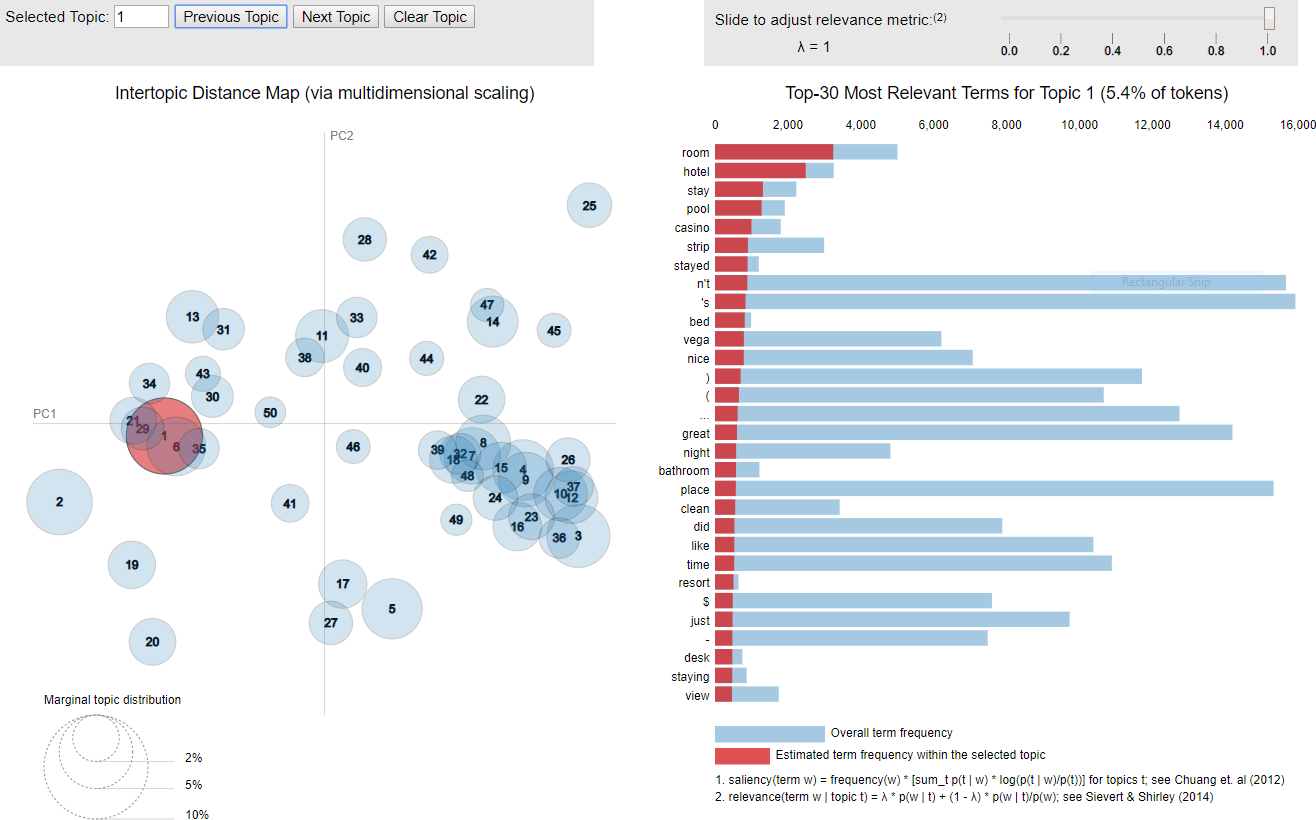
\includegraphics{ntbk-imgs/task01-lda-model-example-hotel.PNG}
\caption{lda-model-example-hotel}
\end{figure}

    \hypertarget{example-topic-suggesting-mexican-cuisine}{%
\subsubsection{Example Topic Suggesting Mexican
Cuisine}\label{example-topic-suggesting-mexican-cuisine}}

\begin{figure}
\centering
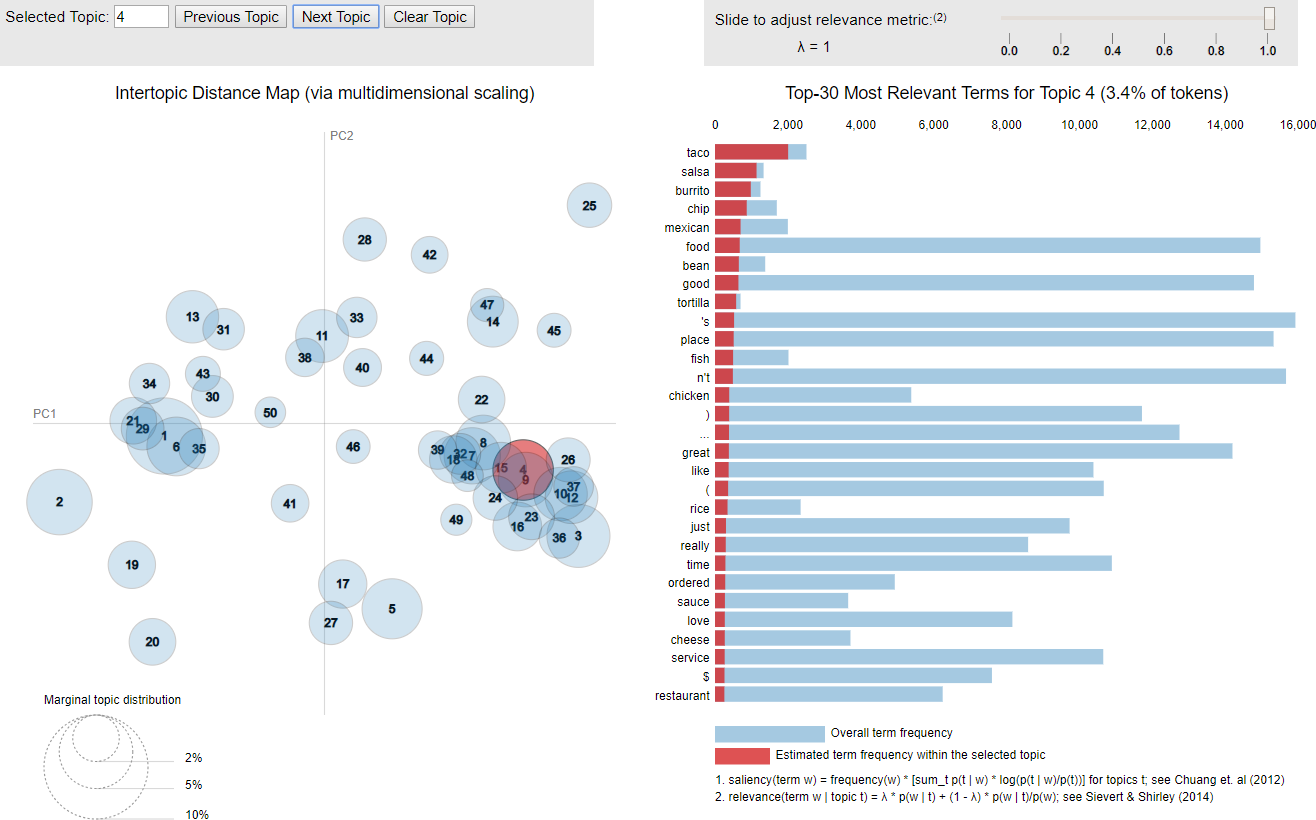
\includegraphics{ntbk-imgs/task01-lda-model-example-mexican-cuisine.PNG}
\caption{lda-model-example-mexican-cuisine}
\end{figure}

    \hypertarget{not-all-topics-make-obvious-sense}{%
\subsection{Not All Topics Make Obvious
Sense}\label{not-all-topics-make-obvious-sense}}

The top terms for a topic do not always suggest a real-world
categorization. The example below includes one or two terms related to
but many more relating to sentiment. I suspect such topics capture terse
reviews such as ``great food'' and ``terrible service.''

\begin{figure}
\centering
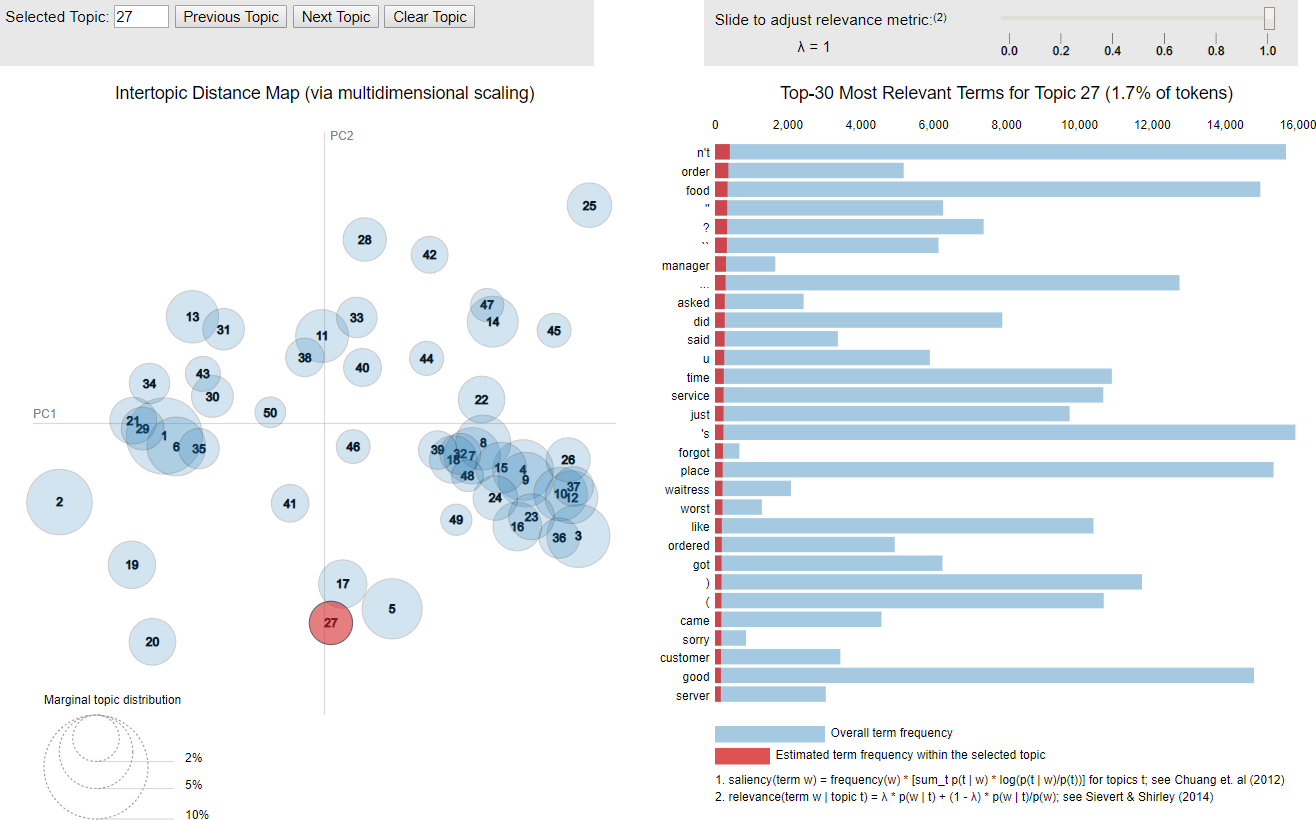
\includegraphics{ntbk-imgs/task01-lda-model-example-unclear.PNG}
\caption{lda-model-example-unclear}
\end{figure}

    \hypertarget{compare-useful-versus-not-useful-reviews}{%
\section{Compare Useful Versus Not Useful
Reviews}\label{compare-useful-versus-not-useful-reviews}}

Each review in the Yelp data set includes votes for cool, funny, and
useful. I thought comparing topics generated from useful versus not
useful would prove\ldots{} useful!

    \begin{Verbatim}[commandchars=\\\{\}]
{\color{incolor}In [{\color{incolor}23}]:} \PY{c+c1}{\PYZsh{} Get indices for Yelp reviws split by useful versus not}
         \PY{c+c1}{\PYZsh{} useful reviews}
         \PY{n}{df}\PY{p}{[}\PY{l+s+s2}{\PYZdq{}}\PY{l+s+s2}{row\PYZus{}num}\PY{l+s+s2}{\PYZdq{}}\PY{p}{]} \PY{o}{=} \PY{n+nb}{range}\PY{p}{(}\PY{n}{df}\PY{o}{.}\PY{n}{shape}\PY{p}{[}\PY{l+m+mi}{0}\PY{p}{]}\PY{p}{)}
         \PY{n}{idxUseful} \PY{o}{=} \PY{n+nb}{list}\PY{p}{(}\PY{n}{df}\PY{p}{[}\PY{l+s+s2}{\PYZdq{}}\PY{l+s+s2}{row\PYZus{}num}\PY{l+s+s2}{\PYZdq{}}\PY{p}{]}\PY{p}{[}\PY{n}{df}\PY{p}{[}\PY{l+s+s2}{\PYZdq{}}\PY{l+s+s2}{votes\PYZus{}useful}\PY{l+s+s2}{\PYZdq{}}\PY{p}{]} \PY{o}{\PYZgt{}} \PY{l+m+mi}{0}\PY{p}{]}\PY{p}{)}
         \PY{n}{idxNotUseful} \PY{o}{=} \PY{n+nb}{list}\PY{p}{(}\PY{n}{df}\PY{p}{[}\PY{l+s+s2}{\PYZdq{}}\PY{l+s+s2}{row\PYZus{}num}\PY{l+s+s2}{\PYZdq{}}\PY{p}{]}\PY{p}{[}\PY{n}{df}\PY{p}{[}\PY{l+s+s2}{\PYZdq{}}\PY{l+s+s2}{votes\PYZus{}useful}\PY{l+s+s2}{\PYZdq{}}\PY{p}{]} \PY{o}{==} \PY{l+m+mi}{0}\PY{p}{]}\PY{p}{)}
\end{Verbatim}


    \begin{Verbatim}[commandchars=\\\{\}]
{\color{incolor}In [{\color{incolor}24}]:} \PY{c+c1}{\PYZsh{} Create separate corpi from useful versus not useful reviews}
         \PY{n}{corpusUseful} \PY{o}{=} \PY{n}{matutils}\PY{o}{.}\PY{n}{Sparse2Corpus}\PY{p}{(}\PY{n}{tokenMatrix}\PY{p}{[}\PY{n}{idxUseful}\PY{p}{,} \PY{p}{:}\PY{p}{]}\PY{p}{,} \PYZbs{}
                                               \PY{n}{documents\PYZus{}columns}\PY{o}{=}\PY{k+kc}{False}\PY{p}{)}
         \PY{n}{corpusNotUseful} \PY{o}{=} \PY{n}{matutils}\PY{o}{.}\PY{n}{Sparse2Corpus}\PY{p}{(}\PY{n}{tokenMatrix}\PY{p}{[}\PY{n}{idxNotUseful}\PY{p}{,} \PY{p}{:}\PY{p}{]}\PY{p}{,} \PYZbs{}
                                                  \PY{n}{documents\PYZus{}columns}\PY{o}{=}\PY{k+kc}{False}\PY{p}{)}
\end{Verbatim}


    \begin{Verbatim}[commandchars=\\\{\}]
{\color{incolor}In [{\color{incolor}25}]:} \PY{c+c1}{\PYZsh{} Print the number of reviews in each corpus}
         \PY{n+nb}{print}\PY{p}{(}\PY{l+s+s2}{\PYZdq{}}\PY{l+s+s2}{The data set has }\PY{l+s+si}{\PYZob{}:,\PYZcb{}}\PY{l+s+s2}{ useful and }\PY{l+s+si}{\PYZob{}:,\PYZcb{}}\PY{l+s+s2}{ not useful reviews.}\PY{l+s+s2}{\PYZdq{}}\PY{o}{.}\PY{n}{format}\PY{p}{(}\PY{n+nb}{len}\PY{p}{(}\PY{n}{corpusUseful}\PY{p}{)}\PY{p}{,} \PY{n+nb}{len}\PY{p}{(}\PY{n}{corpusNotUseful}\PY{p}{)}\PY{p}{)}\PY{p}{)}
\end{Verbatim}


    \begin{Verbatim}[commandchars=\\\{\}]
The data set has 165,231 useful and 172,406 not useful reviews.

    \end{Verbatim}

    The subsets of useful and not useful reviews appear roughly equal. Their
similar size should improve the comparability of the resulting topic
models.

    \hypertarget{find-topics-using-lda}{%
\subsection{Find Topics Using LDA}\label{find-topics-using-lda}}

I stuck with LDA for finding topics in useful and not useful subsets. It
makes results easier to compare to the topics generated from the full
dat set.

    \begin{Verbatim}[commandchars=\\\{\}]
{\color{incolor}In [{\color{incolor}26}]:} \PY{o}{\PYZpc{}\PYZpc{}}\PY{k}{time}
         \PYZpc{}\PYZpc{}capture \PYZhy{}\PYZhy{}no\PYZhy{}stdout
         
         \PYZsh{} Find topics from useful reviews
         print(\PYZdq{}Finding topics from useful reviews...\PYZdq{})
         ldaUseful = models.ldamulticore.LdaMulticore(corpusUseful, \PYZbs{}
                                                      num\PYZus{}topics=num\PYZus{}topics, \PYZbs{}
                                                      id2word=dict(dictionary.items()))
\end{Verbatim}


    \begin{Verbatim}[commandchars=\\\{\}]
Finding topics from useful reviews{\ldots}
CPU times: user 48.6 s, sys: 11.9 s, total: 1min
Wall time: 59.1 s

    \end{Verbatim}

    \begin{Verbatim}[commandchars=\\\{\}]
{\color{incolor}In [{\color{incolor}27}]:} \PY{o}{\PYZpc{}\PYZpc{}}\PY{k}{time}
         \PYZpc{}\PYZpc{}capture \PYZhy{}\PYZhy{}no\PYZhy{}stdout
         
         \PYZsh{} Find topics from not useful reviews
         print(\PYZdq{}Finding topics from not useful reviews...\PYZdq{})
         ldaNotUseful = models.ldamulticore.LdaMulticore(corpusNotUseful, \PYZbs{}
                                                         num\PYZus{}topics=num\PYZus{}topics,
                                                         id2word=dict(dictionary.items()))
\end{Verbatim}


    \begin{Verbatim}[commandchars=\\\{\}]
Finding topics from not useful reviews{\ldots}
CPU times: user 30.6 s, sys: 9.11 s, total: 39.8 s
Wall time: 39.1 s

    \end{Verbatim}

    \hypertarget{graph-terms-topics-and-models}{%
\subsection{Graph Terms, Topics, and
Models}\label{graph-terms-topics-and-models}}

The \href{https://github.com/bmabey/pyLDAvis}{pyLDAvis package} does not
help compare different topic models. I instead graphed the top terms
across topics and models. Side-by-side comparison of the term
distributions revealed similarities and differences between models.

    \begin{Verbatim}[commandchars=\\\{\}]
{\color{incolor}In [{\color{incolor}30}]:} \PY{c+c1}{\PYZsh{} Complile a set of all top\PYZhy{}N tokens from each topic}
         \PY{n}{token\PYZus{}set} \PY{o}{=} \PY{n+nb}{set}\PY{p}{(}\PY{p}{)}
         \PY{n}{getTopNTokens} \PY{o}{=} \PY{k}{lambda} \PY{n}{m}\PY{p}{,} \PY{n}{topn}\PY{p}{:} \PY{p}{[}\PY{n}{w}\PY{p}{[}\PY{l+m+mi}{0}\PY{p}{]} \PY{k}{for} \PY{n}{t} \PY{o+ow}{in} \PY{n+nb}{range}\PY{p}{(}\PY{n}{m}\PY{o}{.}\PY{n}{num\PYZus{}topics}\PY{p}{)} \PYZbs{}
                                          \PY{k}{for} \PY{n}{w} \PY{o+ow}{in} \PY{n}{m}\PY{o}{.}\PY{n}{get\PYZus{}topic\PYZus{}terms}\PY{p}{(}\PY{n}{t}\PY{p}{,} \PY{n}{topn}\PY{p}{)}\PY{p}{]}
         \PY{n}{token\PYZus{}set}\PY{o}{.}\PY{n}{update}\PY{p}{(}\PY{n}{getTopNTokens}\PY{p}{(}\PY{n}{ldaUseful}\PY{p}{,} \PY{n}{num\PYZus{}words}\PY{p}{)}\PY{p}{)}
         \PY{n}{token\PYZus{}set}\PY{o}{.}\PY{n}{update}\PY{p}{(}\PY{n}{getTopNTokens}\PY{p}{(}\PY{n}{ldaNotUseful}\PY{p}{,} \PY{n}{num\PYZus{}words}\PY{p}{)}\PY{p}{)}
\end{Verbatim}


    \begin{Verbatim}[commandchars=\\\{\}]
{\color{incolor}In [{\color{incolor}31}]:} \PY{c+c1}{\PYZsh{} Create a dataframe from token IDs to more easily}
         \PY{c+c1}{\PYZsh{} manage related data}
         \PY{n}{dfCompare} \PY{o}{=} \PY{n}{pd}\PY{o}{.}\PY{n}{DataFrame}\PY{p}{(}\PY{n+nb}{list}\PY{p}{(}\PY{n}{token\PYZus{}set}\PY{p}{)}\PY{p}{,} \PY{n}{columns}\PY{o}{=}\PY{p}{[}\PY{l+s+s2}{\PYZdq{}}\PY{l+s+s2}{token\PYZus{}id}\PY{l+s+s2}{\PYZdq{}}\PY{p}{]}\PY{p}{)}
\end{Verbatim}


    \begin{Verbatim}[commandchars=\\\{\}]
{\color{incolor}In [{\color{incolor}32}]:} \PY{c+c1}{\PYZsh{} Add column for token from ID}
         \PY{n}{dfCompare}\PY{p}{[}\PY{l+s+s2}{\PYZdq{}}\PY{l+s+s2}{token}\PY{l+s+s2}{\PYZdq{}}\PY{p}{]} \PY{o}{=} \PY{n}{dfCompare}\PY{o}{.}\PY{n}{token\PYZus{}id}\PY{o}{.}\PY{n}{apply}\PY{p}{(}\PY{k}{lambda} \PY{n}{i}\PY{p}{:} \PY{n}{dictionary}\PY{p}{[}\PY{n}{i}\PY{p}{]}\PY{p}{)}
\end{Verbatim}


    \begin{Verbatim}[commandchars=\\\{\}]
{\color{incolor}In [{\color{incolor}33}]:} \PY{c+c1}{\PYZsh{} Create functions to count number of topics and sum}
         \PY{c+c1}{\PYZsh{} distribution by token}
         \PY{c+c1}{\PYZsh{}}
         \PY{c+c1}{\PYZsh{} Note: Set `minimum\PYZus{}probability` parameter for `get\PYZus{}term\PYZus{}topics`}
         \PY{c+c1}{\PYZsh{} to zero because default must be much higher. Not documented.}
         \PY{n}{countTermTopics} \PY{o}{=} \PY{k}{lambda} \PY{n}{w}\PY{p}{,} \PY{n}{m}\PY{p}{:} \PY{n+nb}{len}\PY{p}{(}\PY{n}{m}\PY{o}{.}\PY{n}{get\PYZus{}term\PYZus{}topics}\PY{p}{(}\PY{n}{w}\PY{p}{,} \PY{l+m+mi}{0}\PY{p}{)}\PY{p}{)}
         \PY{n}{sumTermTopicDist} \PY{o}{=} \PY{k}{lambda} \PY{n}{w}\PY{p}{,} \PY{n}{m}\PY{p}{:} \PY{l+m+mi}{0} \PY{k}{if} \PY{n}{m}\PY{o}{.}\PY{n}{get\PYZus{}term\PYZus{}topics}\PY{p}{(}\PY{n}{w}\PY{p}{,} \PY{l+m+mi}{0}\PY{p}{)} \PY{o+ow}{is} \PY{k+kc}{None} \PY{k}{else} \PYZbs{}
                                         \PY{n+nb}{sum}\PY{p}{(}\PY{p}{[}\PY{n}{t}\PY{p}{[}\PY{l+m+mi}{1}\PY{p}{]} \PY{k}{for} \PY{n}{t} \PY{o+ow}{in} \PY{n}{m}\PY{o}{.}\PY{n}{get\PYZus{}term\PYZus{}topics}\PY{p}{(}\PY{n}{w}\PY{p}{,} \PY{l+m+mi}{0}\PY{p}{)}\PY{p}{]}\PY{p}{)} 
\end{Verbatim}


    \begin{Verbatim}[commandchars=\\\{\}]
{\color{incolor}In [{\color{incolor}34}]:} \PY{c+c1}{\PYZsh{} Add columns counting and summing distributions for}
         \PY{c+c1}{\PYZsh{} useful topics}
         \PY{n}{dfCompare}\PY{p}{[}\PY{l+s+s2}{\PYZdq{}}\PY{l+s+s2}{count\PYZus{}useful}\PY{l+s+s2}{\PYZdq{}}\PY{p}{]} \PY{o}{=} \PY{n}{dfCompare}\PY{o}{.}\PY{n}{token\PYZus{}id}\PY{o}{.}\PY{n}{apply}\PY{p}{(}\PY{k}{lambda} \PY{n}{i}\PY{p}{:} \PY{n}{countTermTopics}\PY{p}{(}\PY{n}{i}\PY{p}{,} \PY{n}{ldaUseful}\PY{p}{)}\PY{p}{)}
         \PY{n}{dfCompare}\PY{p}{[}\PY{l+s+s2}{\PYZdq{}}\PY{l+s+s2}{dist\PYZus{}useful}\PY{l+s+s2}{\PYZdq{}}\PY{p}{]} \PY{o}{=} \PY{n}{dfCompare}\PY{o}{.}\PY{n}{token\PYZus{}id}\PY{o}{.}\PY{n}{apply}\PY{p}{(}\PY{k}{lambda} \PY{n}{i}\PY{p}{:} \PY{n}{sumTermTopicDist}\PY{p}{(}\PY{n}{i}\PY{p}{,} \PY{n}{ldaUseful}\PY{p}{)}\PY{p}{)}
\end{Verbatim}


    \begin{Verbatim}[commandchars=\\\{\}]
{\color{incolor}In [{\color{incolor}35}]:} \PY{c+c1}{\PYZsh{} Add columns counting and summing distributions for}
         \PY{c+c1}{\PYZsh{} not useful topics}
         \PY{n}{dfCompare}\PY{p}{[}\PY{l+s+s2}{\PYZdq{}}\PY{l+s+s2}{count\PYZus{}not\PYZus{}useful}\PY{l+s+s2}{\PYZdq{}}\PY{p}{]} \PY{o}{=} \PY{n}{dfCompare}\PY{o}{.}\PY{n}{token\PYZus{}id}\PY{o}{.}\PY{n}{apply}\PY{p}{(}\PY{k}{lambda} \PY{n}{i}\PY{p}{:} \PY{n}{countTermTopics}\PY{p}{(}\PY{n}{i}\PY{p}{,} \PY{n}{ldaNotUseful}\PY{p}{)}\PY{p}{)}
         \PY{n}{dfCompare}\PY{p}{[}\PY{l+s+s2}{\PYZdq{}}\PY{l+s+s2}{dist\PYZus{}not\PYZus{}useful}\PY{l+s+s2}{\PYZdq{}}\PY{p}{]} \PY{o}{=} \PY{n}{dfCompare}\PY{o}{.}\PY{n}{token\PYZus{}id}\PY{o}{.}\PY{n}{apply}\PY{p}{(}\PY{k}{lambda} \PY{n}{i}\PY{p}{:} \PY{n}{sumTermTopicDist}\PY{p}{(}\PY{n}{i}\PY{p}{,} \PY{n}{ldaNotUseful}\PY{p}{)}\PY{p}{)}
\end{Verbatim}


    \begin{Verbatim}[commandchars=\\\{\}]
{\color{incolor}In [{\color{incolor}36}]:} \PY{c+c1}{\PYZsh{} Set tokens and reset index}
         \PY{n}{dfCompare}\PY{o}{.}\PY{n}{sort\PYZus{}values}\PY{p}{(}\PY{l+s+s2}{\PYZdq{}}\PY{l+s+s2}{token}\PY{l+s+s2}{\PYZdq{}}\PY{p}{,} \PY{n}{ascending}\PY{o}{=}\PY{k+kc}{False}\PY{p}{,} \PY{n}{inplace}\PY{o}{=}\PY{k+kc}{True}\PY{p}{)}
         \PY{n}{dfCompare}\PY{o}{.}\PY{n}{reset\PYZus{}index}\PY{p}{(}\PY{n}{drop}\PY{o}{=}\PY{k+kc}{True}\PY{p}{,} \PY{n}{inplace}\PY{o}{=}\PY{k+kc}{True}\PY{p}{)}
\end{Verbatim}


    \begin{Verbatim}[commandchars=\\\{\}]
{\color{incolor}In [{\color{incolor}41}]:} \PY{c+c1}{\PYZsh{} A single chart, while easier to view in Jupyter, looks terrible}
         \PY{c+c1}{\PYZsh{} as a PDF. The helper function below will create the same chart}
         \PY{c+c1}{\PYZsh{} for a subset of tokens.}
         \PY{k}{def} \PY{n+nf}{splitGraph}\PY{p}{(}\PY{n}{startTokenID}\PY{p}{,} \PY{n}{endTokenID}\PY{p}{)}\PY{p}{:}
             \PY{l+s+sd}{\PYZdq{}\PYZdq{}\PYZdq{}Create chart for subset of useful versus not useful term\PYZhy{}topic distribution\PYZdq{}\PYZdq{}\PYZdq{}}
             \PY{n}{fig}\PY{p}{,} \PY{n}{ax} \PY{o}{=} \PY{n}{plot}\PY{o}{.}\PY{n}{subplots}\PY{p}{(}\PY{p}{)}
             \PY{n}{fig}\PY{o}{.}\PY{n}{set\PYZus{}size\PYZus{}inches}\PY{p}{(}\PY{l+m+mi}{8}\PY{p}{,} \PY{l+m+mi}{11}\PY{p}{)}
         
             \PY{c+c1}{\PYZsh{} Add horizontal bars}
             \PY{n}{index} \PY{o}{=} \PY{n}{np}\PY{o}{.}\PY{n}{array}\PY{p}{(}\PY{n}{dfCompare}\PY{o}{.}\PY{n}{index}\PY{p}{)}\PY{p}{[}\PY{n}{startTokenID}\PY{p}{:}\PY{n}{endTokenID}\PY{p}{]}
             \PY{n}{width} \PY{o}{=} \PY{l+m+mf}{0.5}
             \PY{n}{gap} \PY{o}{=} \PY{n}{width} \PY{o}{/} \PY{l+m+mi}{5}
             \PY{n}{barsUseful} \PY{o}{=} \PY{n}{ax}\PY{o}{.}\PY{n}{barh}\PY{p}{(}\PY{n}{index}\PY{o}{+}\PY{n}{width}\PY{p}{,} \PYZbs{}
                                  \PY{n+nb}{list}\PY{p}{(}\PY{n}{dfCompare}\PY{o}{.}\PY{n}{dist\PYZus{}useful}\PY{p}{)}\PY{p}{[}\PY{n}{startTokenID}\PY{p}{:}\PY{n}{endTokenID}\PY{p}{]}\PY{p}{,} \PYZbs{}
                                  \PY{n}{width}\PY{o}{\PYZhy{}}\PY{n}{gap}\PY{p}{,} \PY{n}{label}\PY{o}{=}\PY{l+s+s2}{\PYZdq{}}\PY{l+s+s2}{Useful Reviews}\PY{l+s+s2}{\PYZdq{}}\PY{p}{,} \PY{n}{align}\PY{o}{=}\PY{l+s+s2}{\PYZdq{}}\PY{l+s+s2}{edge}\PY{l+s+s2}{\PYZdq{}}\PY{p}{,} \PYZbs{}
                                  \PY{n}{color}\PY{o}{=}\PY{l+s+s2}{\PYZdq{}}\PY{l+s+s2}{\PYZsh{}cc474d}\PY{l+s+s2}{\PYZdq{}}\PY{p}{)}
             \PY{n}{barsNotUseful} \PY{o}{=} \PY{n}{ax}\PY{o}{.}\PY{n}{barh}\PY{p}{(}\PY{n}{index}\PY{o}{+}\PY{n}{gap}\PY{p}{,}
                                     \PY{n+nb}{list}\PY{p}{(}\PY{n}{dfCompare}\PY{o}{.}\PY{n}{dist\PYZus{}not\PYZus{}useful}\PY{p}{)}\PY{p}{[}\PY{n}{startTokenID}\PY{p}{:}\PY{n}{endTokenID}\PY{p}{]}\PY{p}{,} \PYZbs{}
                                     \PY{n}{width}\PY{o}{\PYZhy{}}\PY{n}{gap}\PY{p}{,} \PY{n}{label}\PY{o}{=}\PY{l+s+s2}{\PYZdq{}}\PY{l+s+s2}{Not Useful Reviews}\PY{l+s+s2}{\PYZdq{}}\PY{p}{,} \PY{n}{align}\PY{o}{=}\PY{l+s+s2}{\PYZdq{}}\PY{l+s+s2}{edge}\PY{l+s+s2}{\PYZdq{}}\PY{p}{,} \PYZbs{}
                                     \PY{n}{color}\PY{o}{=}\PY{l+s+s2}{\PYZdq{}}\PY{l+s+s2}{\PYZsh{}a5c9e1}\PY{l+s+s2}{\PYZdq{}}\PY{p}{)}
         
             \PY{c+c1}{\PYZsh{} Configure horizontal axis at top}
             \PY{n}{ax}\PY{o}{.}\PY{n}{set\PYZus{}xlabel}\PY{p}{(}\PY{l+s+s2}{\PYZdq{}}\PY{l+s+s2}{Term Distribution Across Topics}\PY{l+s+s2}{\PYZdq{}}\PY{p}{)}
             \PY{n}{ax}\PY{o}{.}\PY{n}{xaxis}\PY{o}{.}\PY{n}{set\PYZus{}label\PYZus{}position}\PY{p}{(}\PY{l+s+s2}{\PYZdq{}}\PY{l+s+s2}{top}\PY{l+s+s2}{\PYZdq{}}\PY{p}{)}
             \PY{n}{ax}\PY{o}{.}\PY{n}{xaxis}\PY{o}{.}\PY{n}{tick\PYZus{}top}\PY{p}{(}\PY{p}{)}
         
             \PY{c+c1}{\PYZsh{} Configure vertical axis with token labels}
             \PY{n}{ax}\PY{o}{.}\PY{n}{set\PYZus{}ylabel}\PY{p}{(}\PY{l+s+s2}{\PYZdq{}}\PY{l+s+s2}{Tokens}\PY{l+s+s2}{\PYZdq{}}\PY{p}{)}
         \PY{c+c1}{\PYZsh{}     ax.set\PYZus{}ylim(2*width\PYZhy{}1, len(index))}
             \PY{n}{plot}\PY{o}{.}\PY{n}{yticks}\PY{p}{(}\PY{n}{index}\PY{o}{+}\PY{n}{width}\PY{p}{,} \PY{n}{dfCompare}\PY{o}{.}\PY{n}{token}\PY{p}{[}\PY{n}{startTokenID}\PY{p}{:}\PY{n}{endTokenID}\PY{p}{]}\PY{p}{)}
         
             \PY{c+c1}{\PYZsh{} Enable legend}
             \PY{n}{ax}\PY{o}{.}\PY{n}{legend}\PY{p}{(}\PY{n}{loc}\PY{o}{=}\PY{l+m+mi}{1}\PY{p}{)}
         
             \PY{c+c1}{\PYZsh{} Return plot}
             \PY{k}{return} \PY{n}{plot}
\end{Verbatim}


    \begin{Verbatim}[commandchars=\\\{\}]
{\color{incolor}In [{\color{incolor}42}]:} \PY{c+c1}{\PYZsh{} First subset}
         \PY{n}{step} \PY{o}{=} \PY{n+nb}{int}\PY{p}{(}\PY{n}{dfCompare}\PY{o}{.}\PY{n}{shape}\PY{p}{[}\PY{l+m+mi}{0}\PY{p}{]} \PY{o}{/} \PY{l+m+mi}{3}\PY{p}{)}
         \PY{n}{stop} \PY{o}{=} \PY{n}{dfCompare}\PY{o}{.}\PY{n}{shape}\PY{p}{[}\PY{l+m+mi}{0}\PY{p}{]}
         \PY{n}{start} \PY{o}{=} \PY{n}{stop} \PY{o}{\PYZhy{}} \PY{n}{step}
         \PY{n}{plot}\PY{o}{.}\PY{n}{show}\PY{p}{(}\PY{n}{splitGraph}\PY{p}{(}\PY{n}{start}\PY{p}{,} \PY{n}{stop}\PY{p}{)}\PY{p}{)}
\end{Verbatim}


    \begin{center}
    \adjustimage{max size={0.9\linewidth}{0.9\paperheight}}{output_51_0.png}
    \end{center}
    { \hspace*{\fill} \\}
    
    \begin{Verbatim}[commandchars=\\\{\}]
{\color{incolor}In [{\color{incolor}43}]:} \PY{c+c1}{\PYZsh{} Second subset}
         \PY{n}{stop} \PY{o}{=} \PY{n}{start}
         \PY{n}{start} \PY{o}{=} \PY{n}{stop} \PY{o}{\PYZhy{}} \PY{n}{step}
         \PY{n}{plot}\PY{o}{.}\PY{n}{show}\PY{p}{(}\PY{n}{splitGraph}\PY{p}{(}\PY{n}{start}\PY{p}{,} \PY{n}{stop}\PY{p}{)}\PY{p}{)}
\end{Verbatim}


    \begin{center}
    \adjustimage{max size={0.9\linewidth}{0.9\paperheight}}{output_52_0.png}
    \end{center}
    { \hspace*{\fill} \\}
    
    \begin{Verbatim}[commandchars=\\\{\}]
{\color{incolor}In [{\color{incolor}44}]:} \PY{c+c1}{\PYZsh{} Third (final) subset}
         \PY{n}{stop} \PY{o}{=} \PY{n}{start}
         \PY{n}{start} \PY{o}{=} \PY{l+m+mi}{0}
         \PY{n}{plot}\PY{o}{.}\PY{n}{show}\PY{p}{(}\PY{n}{splitGraph}\PY{p}{(}\PY{n}{start}\PY{p}{,} \PY{n}{stop}\PY{p}{)}\PY{p}{)}
\end{Verbatim}


    \begin{center}
    \adjustimage{max size={0.9\linewidth}{0.9\paperheight}}{output_53_0.png}
    \end{center}
    { \hspace*{\fill} \\}
    
    The resulting models are similar but not identical. They differ most
significantly on semantic words like ``good'' and ``love''. They also
differ on low-utility words like ``place''. Interestingly, the not
useful reviews include both low-utility \emph{and semantic} words as a
higher proportion of their topic distributions.

The higher proportion of low-utilitly words makes sense; generic reviews
should garner few votes for usefulness. I do not fully understand the
higher proportion of semantic words. Perhaps the difference relates to
my earlier supposition on ``terse'' reviews. Such reviews (e.g., ``great
food'' and ``terrible service'') might receive fewer votes as useful.


    % Add a bibliography block to the postdoc
    
    
    
    \end{document}
